% !TEX spellcheck = en_US



% ~~~~~~~~~~~~~~~~~~~~~~~~~~~~~~~~~~~~~~~ V
% (NC) 2026 Haluk Bingol
% github.com/halukbingol/LaTeX-Templates
%
% Licensees may copy, distribute, display, and perform the work and make derivative works 
% and remixes based on it only for non-commercial purposes. 
% ~~~~~~~~~~~~~~~~~~~~~~~~~~~~~~~~~~~~~~~ A




% =====================================================================
%  Maven for Java -- Concepts: Builds, Coordinates, Repositories, Dependencies and the Lifecycle
%  ---------------------------------------------------------------------
%  Built on hblib/Template/hblibTemplate.tex with the libraries in ../../hblib/.
%  Programs and their real outputs are in codeoutput/:
%     codeoutput/<Name>.java  a program (classes without main() are only compiled)
%     codeoutput/<Name>.sh    a terminal session, run in a copy of codeoutput/<Name>/
%     codeoutput/<Name>.txt   what it printed, made by:  bash run_examples.sh
% =====================================================================

\documentclass[aspectratio=169,10pt,compress]{beamer}

% ~~~~~~~~~~~~~~~~~~~~~~~~~~~~~~~~~~~~~~~~~~~~~~~~~~~~~~~~~~~~~~~~~ V hblib
	\usepackage{../../hblib/hblibPresentation} % lib presentation: theme, i/N, \hSection, algorithm2e, ...
	\usepackage{../../hblib/hblibCodeoutput} % lib code + output: \lstcode, \lstterminal, ...
	\usepackage{../../hblib/hblibDatastructures} % lib data structures: \hString, \hStack, \hQueue
% ~~~~~~~~~~~~~~~~~~~~~~~~~~~~~~~~~~~~~~~~~~~~~~~~~~~~~~~~~~~~~~~~~ A hblib


% theme, i/N, fonts (T1, lmodern), booktabs, xcolor, array (L{width} columns), listings, tikz,
% algorithm2e (\small captions, \Fn) and the color gitred come from the hblib libraries




% +++++++++++++++++++++++++++++++++++++++ V specific
\DontPrintSemicolon % in algorithms
\newcommand{\win}{\textbf{Windows}}
\newcommand{\mac}{\textbf{macOS}}
\usetikzlibrary{positioning}
% +++++++++++++++++++++++++++++++++++++++ A specific

% ---------------------------------------------------------------------
\title{Maven for Java}
\subtitle{Concepts: Builds, Coordinates, Repositories, Dependencies and the Lifecycle}
\author[Bingol]{Haluk O. Bingol}

\institute[FCIS]{
    Faculty of Computer and Information Sciences\\
    Yeditepe University
}
\date{
	{\tiny \hbTimeStamp}
}

\begin{document}




% ~~~~~~~~~~~~~~~~~~~~~~~~~~~~~~~~~~~~~~ V frm
\begin{frame}[t,fragile]
  \titlepage
\end{frame}
% ~~~~~~~~~~~~~~~~~~~~~~~~~~~~~~~~~~~~~~ A frm




% ~~~~~~~~~~~~~~~~~~~~~~~~~~~~~~~~~~~~~~ V frm
\begin{frame}[t,fragile] \frametitle{Outline}
  \begin{columns}[T]
    \begin{column}{0.48\textwidth}
      \tableofcontents[sections={1-5}, hideallsubsections]
    \end{column}
    \begin{column}{0.48\textwidth}
      \tableofcontents[sections={6-10}, hideallsubsections]
    \end{column}
  \end{columns}
\end{frame}
% ~~~~~~~~~~~~~~~~~~~~~~~~~~~~~~~~~~~~~~ A frm

% ~~~~~~~~~~~~~~~~~~~~~~~~~~~~~~~~~~~~~~ V
\hSection[Builds]{What Is a Build?}
% ~~~~~~~~~~~~~~~~~~~~~~~~~~~~~~~~~~~~~~ A




% ~~~~~~~~~~~~~~~~~~~~~~~~~~~~~~~~~~~~~~ V frm
\begin{frame}[t,fragile] \frametitle{From sources to something that runs}
  \begin{center}
  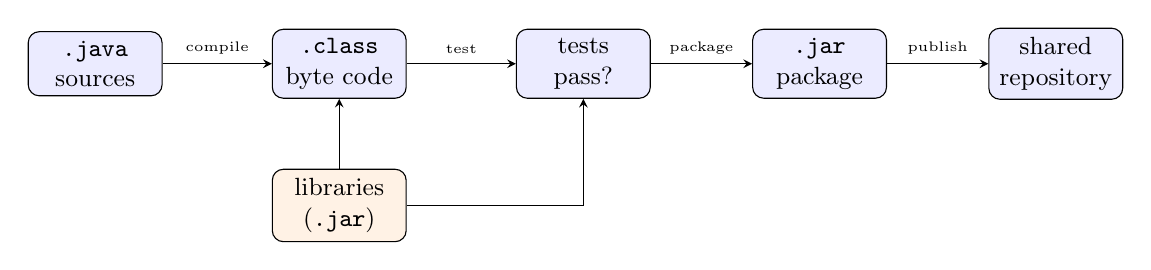
\begin{tikzpicture}[box/.style={draw, rounded corners, fill=blue!8, font=\small, minimum width=1.7cm, minimum height=0.8cm, align=center}, >=stealth]
    \node[box] (s) at (0,0)     {\texttt{.java}\\sources};
    \node[box] (c) at (3.1,0)   {\texttt{.class}\\byte code};
    \node[box] (t) at (6.2,0)   {tests\\pass?};
    \node[box] (j) at (9.2,0)   {\texttt{.jar}\\package};
    \node[box] (r) at (12.2,0)  {shared\\repository};
    \node[box, fill=orange!10] (l) at (3.1,-1.8) {libraries\\(\texttt{.jar})};
    \draw[->] (s) -- node[above, font=\tiny] {compile} (c);
    \draw[->] (c) -- node[above, font=\tiny] {test} (t);
    \draw[->] (t) -- node[above, font=\tiny] {package} (j);
    \draw[->] (j) -- node[above, font=\tiny] {publish} (r);
    \draw[->] (l) -- (c);
    \draw[->] (l) -| (t);
  \end{tikzpicture}
  \end{center}
  \begin{itemize}\small
    \item A \textbf{build} turns sources into a tested, packaged, shareable product.
    \item Each step needs the right libraries in the right versions: the \textbf{class path}.
    \item A \textbf{build tool} does all steps the same way every time, on every computer.
  \end{itemize}
\end{frame}
% ~~~~~~~~~~~~~~~~~~~~~~~~~~~~~~~~~~~~~~ A frm




% ~~~~~~~~~~~~~~~~~~~~~~~~~~~~~~~~~~~~~~ V frm
\begin{frame}[t,fragile] \frametitle{A short history of Java build tools}
  \begin{center}\small
  \begin{tabular}{@{}llL{0.6\textwidth}@{}}
    \toprule
    \textbf{year} & \textbf{tool}  & \textbf{idea} \\
    \midrule
    1976 & make            & rules: a target, the files it depends on, the commands (C programs) \\
    2000 & Apache Ant      & \texttt{make} for Java in XML; every step written by hand \\
    2004 & Apache Maven 1  & a project \emph{model}: conventions, a lifecycle, downloaded dependencies \\
    2005 & Maven 2         & transitive dependencies, Maven Central as we know it \\
    2010 & Maven 3         & today's line: 3.10.0 is the current release (September 2026) \\
    2012 & Gradle 1.0      & builds as code (Groovy, later Kotlin), Maven's repositories \\
    2026 & Maven 4         & release candidates (4.0.0-rc-7, September 2026) \\
    \bottomrule
  \end{tabular}
  \end{center}
  \small All of them still exist; for Java, Maven and Gradle are the common choices, and they share the repositories.
\end{frame}
% ~~~~~~~~~~~~~~~~~~~~~~~~~~~~~~~~~~~~~~ A frm

% ~~~~~~~~~~~~~~~~~~~~~~~~~~~~~~~~~~~~~~ V
\hSection[Layout]{Convention over Configuration}
% ~~~~~~~~~~~~~~~~~~~~~~~~~~~~~~~~~~~~~~ A




% ~~~~~~~~~~~~~~~~~~~~~~~~~~~~~~~~~~~~~~ V frm
\begin{frame}[t,fragile] \frametitle{Agree on a layout, write less}
  \begin{columns}[T]
    \begin{column}{0.44\textwidth}


% +++++++++++++++++++++++++++++++++++++++ V lst
%: -Lst.
\begin{lstlisting}[style=codesnippet, language={}, basicstyle=\ttfamily\footnotesize]
my-app/
  pom.xml
  src/
    main/
      java/         the program
      resources/    files for it
    test/
      java/         the tests
      resources/    files for them
  target/           everything built
\end{lstlisting}
% +++++++++++++++++++++++++++++++++++++++ A lst


    \end{column}
    \begin{column}{0.52\textwidth}
      \begin{itemize}\small
        \item Maven \emph{knows} where things are: no configuration needed for the usual case.
        \item Any Maven project looks the same: a new team member finds the tests at once.
        \item \texttt{target/} is generated: never edit it, never commit it.
        \item You \emph{can} change the defaults; it is rarely worth it.
      \end{itemize}
    \end{column}
  \end{columns}
\end{frame}
% ~~~~~~~~~~~~~~~~~~~~~~~~~~~~~~~~~~~~~~ A frm

% ~~~~~~~~~~~~~~~~~~~~~~~~~~~~~~~~~~~~~~ V
\hSection[GAV]{Coordinates}
% ~~~~~~~~~~~~~~~~~~~~~~~~~~~~~~~~~~~~~~ A




% ~~~~~~~~~~~~~~~~~~~~~~~~~~~~~~~~~~~~~~ V frm
\begin{frame}[t,fragile] \frametitle{Every artifact has an address}
  \begin{itemize}\small
    \item An \textbf{artifact}: a file Maven makes or uses (\texttt{.jar}, \texttt{.pom}, \texttt{.war}).
    \item Its \textbf{coordinates}: \texttt{groupId} (organization, reversed domain), \texttt{artifactId} (name), \texttt{version}; optionally packaging and classifier (\texttt{sources}, \texttt{javadoc}).
    \item The coordinates are also its path in every repository:
  \end{itemize}
  \[
  	\begin{array}{c}
  		\underbrace{\texttt{org.apache.commons}}_{\mathit{groupId}} : \underbrace{\texttt{commons-lang3}}_{\mathit{artifactId}} : \underbrace{\texttt{3.14.0}}_{\mathit{version}} \\
  		\big\downarrow \\
  		\texttt{org/apache/commons/commons-lang3/3.14.0/commons-lang3-3.14.0.jar}
  	\end{array}
  \]
  \begin{itemize}\small
    \item Versions: \texttt{1.0} (release, never changes), \texttt{1.0-SNAPSHOT} (work in progress, changes).
    \item Same coordinates $\Rightarrow$ same file, for everybody, forever (for releases).
  \end{itemize}
\end{frame}
% ~~~~~~~~~~~~~~~~~~~~~~~~~~~~~~~~~~~~~~ A frm

% ~~~~~~~~~~~~~~~~~~~~~~~~~~~~~~~~~~~~~~ V
\hSection[Repos]{Repositories}
% ~~~~~~~~~~~~~~~~~~~~~~~~~~~~~~~~~~~~~~ A




% ~~~~~~~~~~~~~~~~~~~~~~~~~~~~~~~~~~~~~~ V frm
\begin{frame}[t,fragile] \frametitle{Where artifacts live}
  \begin{columns}[T]
    \begin{column}{0.5\textwidth}
      \begin{center}
      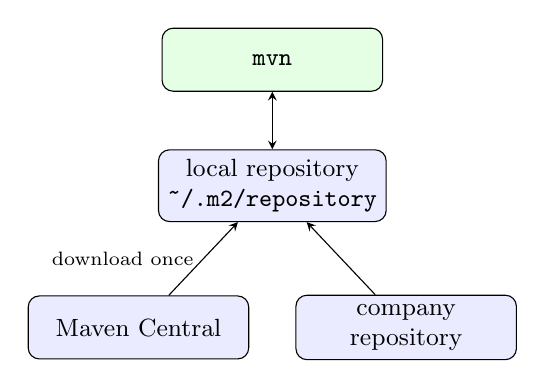
\begin{tikzpicture}[box/.style={draw, rounded corners, fill=blue!8, font=\small, minimum width=2.8cm, minimum height=0.8cm, align=center}, >=stealth]
        \node[box, fill=green!10] (m) at (0,0)    {\texttt{mvn}};
        \node[box] (l) at (0,-1.6) {local repository\\\texttt{\textasciitilde/.m2/repository}};
        \node[box] (c) at (-1.7,-3.4) {Maven Central};
        \node[box] (k) at (1.7,-3.4)  {company\\repository};
        \draw[<->] (m) -- (l);
        \draw[<-] (l) -- node[left, font=\scriptsize] {download once} (c);
        \draw[<-] (l) -- (k);
      \end{tikzpicture}
      \end{center}
    \end{column}
    \begin{column}{0.46\textwidth}
      \begin{itemize}\small
        \item \textbf{Local}: a cache on your computer, shared by all your projects.
        \item \textbf{Remote}: Maven Central (public, the default), company repositories (Nexus, Artifactory).
        \item Missing locally $\Rightarrow$ downloaded once, then reused, also offline.
        \item \texttt{mvn install} puts your own artifact in the local repository; \texttt{mvn deploy} in a remote one.
      \end{itemize}
    \end{column}
  \end{columns}
\end{frame}
% ~~~~~~~~~~~~~~~~~~~~~~~~~~~~~~~~~~~~~~ A frm

% ~~~~~~~~~~~~~~~~~~~~~~~~~~~~~~~~~~~~~~ V
\hSection[Deps]{Dependencies}
% ~~~~~~~~~~~~~~~~~~~~~~~~~~~~~~~~~~~~~~ A




% ~~~~~~~~~~~~~~~~~~~~~~~~~~~~~~~~~~~~~~ V frm
\begin{frame}[t,fragile] \frametitle{Dependencies form a graph}
  \begin{columns}[T]
    \begin{column}{0.5\textwidth}
      \begin{center}
      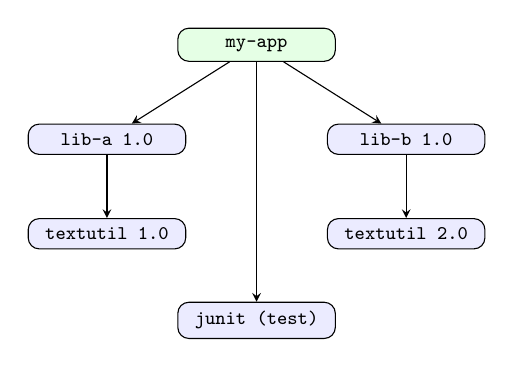
\begin{tikzpicture}[box/.style={draw, rounded corners, fill=blue!8, font=\scriptsize\ttfamily, minimum width=2cm}, >=stealth]
        \node[box, fill=green!10] (p) at (0,0)      {my-app};
        \node[box] (a) at (-1.9,-1.2) {lib-a 1.0};
        \node[box] (b) at (1.9,-1.2)  {lib-b 1.0};
        \node[box] (u1) at (-1.9,-2.4) {textutil 1.0};
        \node[box] (u2) at (1.9,-2.4)  {textutil 2.0};
        \node[box] (j) at (0,-3.5)    {junit (test)};
        \draw[->] (p) -- (a); \draw[->] (p) -- (b);
        \draw[->] (a) -- (u1); \draw[->] (b) -- (u2);
        \draw[->] (p) -- (j);
      \end{tikzpicture}
      \end{center}
    \end{column}
    \begin{column}{0.46\textwidth}
      \begin{itemize}\small
        \item You list \textbf{direct} dependencies; Maven reads their POMs and finds the \textbf{transitive} ones.
        \item A \textbf{scope} says where a dependency is needed: \texttt{compile}, \texttt{test}, \texttt{runtime}, \texttt{provided}.
        \item Two versions of one artifact: only one can be on the class path. Maven picks the \emph{nearest} (senior level).
      \end{itemize}
    \end{column}
  \end{columns}
\end{frame}
% ~~~~~~~~~~~~~~~~~~~~~~~~~~~~~~~~~~~~~~ A frm

% ~~~~~~~~~~~~~~~~~~~~~~~~~~~~~~~~~~~~~~ V
\hSection[Lifecycle]{The Lifecycle}
% ~~~~~~~~~~~~~~~~~~~~~~~~~~~~~~~~~~~~~~ A




% ~~~~~~~~~~~~~~~~~~~~~~~~~~~~~~~~~~~~~~ V frm
\begin{frame}[t,fragile] \frametitle{Phases in a fixed order}
  \begin{center}
  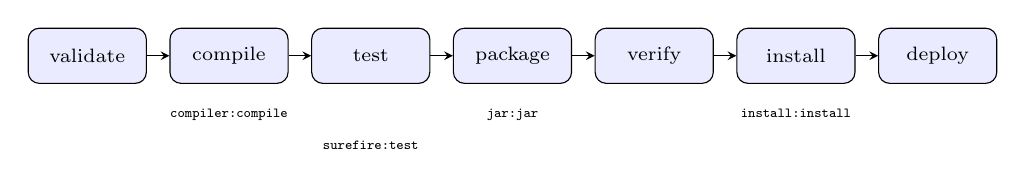
\begin{tikzpicture}[ph/.style={draw, rounded corners, fill=blue!8, font=\scriptsize, minimum width=1.5cm, minimum height=0.7cm}, >=stealth]
    \foreach \p/\x in {validate/0, compile/1.8, test/3.6, package/5.4, verify/7.2, install/9, deploy/10.8} {
      \node[ph] (\p) at (\x,0) {\p};
    }
    \foreach \a/\b in {validate/compile, compile/test, test/package, package/verify, verify/install, install/deploy} {
      \draw[->] (\a) -- (\b);
    }
    \node[font=\tiny\ttfamily, below=0.2cm of compile] {compiler:compile};
    \node[font=\tiny\ttfamily, below=0.6cm of test] {surefire:test};
    \node[font=\tiny\ttfamily, below=0.2cm of package] {jar:jar};
    \node[font=\tiny\ttfamily, below=0.2cm of install] {install:install};
  \end{tikzpicture}
  \end{center}
  \begin{itemize}\small
    \item The \textbf{default lifecycle} (main phases above); also \texttt{clean} and \texttt{site}.
    \item A \textbf{plugin} does the work; its \textbf{goals} (\texttt{plugin:goal}) are \emph{bound} to phases.
    \item \texttt{mvn package} runs every phase up to \texttt{package}, in order. You never say \emph{how}, only \emph{how far}.
  \end{itemize}
\end{frame}
% ~~~~~~~~~~~~~~~~~~~~~~~~~~~~~~~~~~~~~~ A frm




% ~~~~~~~~~~~~~~~~~~~~~~~~~~~~~~~~~~~~~~ V frm
\begin{frame}[t,fragile] \frametitle{What \texttt{mvn <phase>} does}
  \begin{columns}[T]
    \begin{column}{0.56\textwidth}


% +++++++++++++++++++++++++++++++++++++++ V alg
%: -Alg. 
\begin{algorithm}[H]
  \caption{One Maven run}
  \KwIn{a target phase $p$, the projects $P_{1}, \dots, P_{m}$}
  read all POMs; compute each effective POM\;
  sort the projects by their dependencies\tcp*{reactor order}
  \ForEach{project $P_{i}$ in that order}{
    resolve its dependencies (local, then remote)\;
    \ForEach{phase $q$ of the lifecycle up to $p$}{
      run the goals bound to $q$\;
      \lIf{a goal fails}{stop: \texttt{BUILD FAILURE}}
    }
  }
  report \texttt{BUILD SUCCESS}\;
\end{algorithm}
% +++++++++++++++++++++++++++++++++++++++ A alg

    \end{column}
    \begin{column}{0.4\textwidth}
      \begin{itemize}\small
        \item Several projects (modules) in one run: the \textbf{reactor}.
        \item A phase with no goal bound simply does nothing.
        \item A failing test stops the run before \texttt{package}: no untested jar.
      \end{itemize}
    \end{column}
  \end{columns}
\end{frame}
% ~~~~~~~~~~~~~~~~~~~~~~~~~~~~~~~~~~~~~~ A frm

% ~~~~~~~~~~~~~~~~~~~~~~~~~~~~~~~~~~~~~~ V
\hSection[POM]{The Project Object Model}
% ~~~~~~~~~~~~~~~~~~~~~~~~~~~~~~~~~~~~~~ A




% ~~~~~~~~~~~~~~~~~~~~~~~~~~~~~~~~~~~~~~ V frm
\begin{frame}[t,fragile] \frametitle{\texttt{pom.xml}: a description, not a script}
  \begin{columns}[T]
    \begin{column}{0.5\textwidth}
      \begin{itemize}\small
        \item \textbf{What} the project is: coordinates, packaging (\texttt{jar}, \texttt{war}, \texttt{pom}).
        \item \textbf{What it needs}: dependencies with scopes.
        \item \textbf{How it differs} from the conventions: plugin configuration, properties.
        \item \textbf{Inheritance}: a POM can have a parent; all inherit from the Super POM inside Maven.
        \item \textbf{Aggregation}: a parent can list modules built together.
      \end{itemize}
    \end{column}
    \begin{column}{0.46\textwidth}
      \begin{center}
      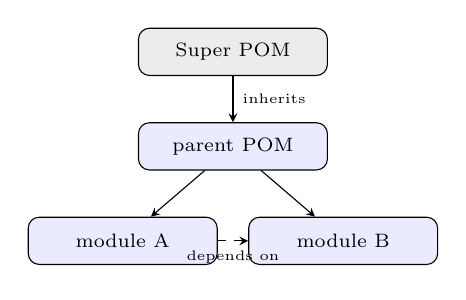
\begin{tikzpicture}[box/.style={draw, rounded corners, fill=blue!8, font=\scriptsize, minimum width=2.4cm, minimum height=0.6cm}, >=stealth]
        \node[box, fill=gray!15] (s) at (0,0)      {Super POM};
        \node[box] (p) at (0,-1.2)                 {parent POM};
        \node[box] (a) at (-1.4,-2.4)              {module A};
        \node[box] (b) at (1.4,-2.4)               {module B};
        \draw[->] (s) -- node[right, font=\tiny] {inherits} (p);
        \draw[->] (p) -- (a); \draw[->] (p) -- (b);
        \draw[->, dashed] (a) -- node[below, font=\tiny] {depends on} (b);
      \end{tikzpicture}
      \end{center}
    \end{column}
  \end{columns}
\end{frame}
% ~~~~~~~~~~~~~~~~~~~~~~~~~~~~~~~~~~~~~~ A frm




% ~~~~~~~~~~~~~~~~~~~~~~~~~~~~~~~~~~~~~~ V frm
\begin{frame}[t,fragile] \frametitle{The smallest real example}
  \begin{columns}[T]
    \begin{column}{0.5\textwidth}
      \lstcode[basicstyle=\ttfamily\scriptsize]{codeoutput/Tiny/src/main/java/hello/Hello.java}{Java}
    \end{column}
    \begin{column}{0.48\textwidth}
      \uncover<2->{\lstterminal[basicstyle=\ttfamily\tiny]{codeoutput/Tiny.txt}}
    \end{column}
  \end{columns}

  \vspace{0.1em}
  \small
  A layout, a \texttt{pom.xml}, one command; \texttt{-q} shows only errors, so nothing at all means success. The POM is shown in the freshman deck.
\end{frame}
% ~~~~~~~~~~~~~~~~~~~~~~~~~~~~~~~~~~~~~~ A frm

% ~~~~~~~~~~~~~~~~~~~~~~~~~~~~~~~~~~~~~~ V
\hSection[OS]{Maven on Windows and macOS}
% ~~~~~~~~~~~~~~~~~~~~~~~~~~~~~~~~~~~~~~ A




% ~~~~~~~~~~~~~~~~~~~~~~~~~~~~~~~~~~~~~~ V frm
\begin{frame}[t,fragile] \frametitle{The same commands everywhere}
  \begin{itemize}\small
    \item Maven is a Java program: it runs wherever a JDK runs; the POM and the commands are the same.
    \item Differences are those of the shells: path separators, class path separators, quoting.
  \end{itemize}
  \begin{columns}[T]
    \begin{column}{0.48\textwidth}
      \begin{block}{Windows (not run here)}


% +++++++++++++++++++++++++++++++++++++++ V lst
%: -Lst.
\begin{lstlisting}[style=codesnippet, language={}, basicstyle=\ttfamily\scriptsize]
mvn -v
mvn package
java -cp target\hello-1.0.jar hello.Hello
dir %USERPROFILE%\.m2\repository
\end{lstlisting}
% +++++++++++++++++++++++++++++++++++++++ A lst


      \end{block}
    \end{column}
    \begin{column}{0.48\textwidth}
      \begin{block}{macOS (not run here)}


% +++++++++++++++++++++++++++++++++++++++ V lst
%: -Lst.
\begin{lstlisting}[style=codesnippet, language=bash, basicstyle=\ttfamily\scriptsize]
mvn -v
mvn package
java -cp target/hello-1.0.jar hello.Hello
ls ~/.m2/repository
\end{lstlisting}
% +++++++++++++++++++++++++++++++++++++++ A lst


      \end{block}
    \end{column}
  \end{columns}

  \small IDEs (Eclipse, IntelliJ IDEA, VS Code) open \texttt{pom.xml} directly and use the same model.
\end{frame}
% ~~~~~~~~~~~~~~~~~~~~~~~~~~~~~~~~~~~~~~ A frm

% ~~~~~~~~~~~~~~~~~~~~~~~~~~~~~~~~~~~~~~ V
\hSection[Levels]{The Road Ahead}
% ~~~~~~~~~~~~~~~~~~~~~~~~~~~~~~~~~~~~~~ A




% ~~~~~~~~~~~~~~~~~~~~~~~~~~~~~~~~~~~~~~ V frm
\begin{frame}[t,fragile] \frametitle{What each level adds}
  \begin{center}\small
  \begin{tabular}{@{}lL{0.72\textwidth}@{}}
    \toprule
    \textbf{level}  & \textbf{topics} \\
    \midrule
    freshman        & installing, the first project, compile, test, package, clean, reading errors \\
    sophomore       & phases and goals, dependencies and scopes, resources, \texttt{exec}, runnable jars, test options \\
    junior          & modules and the reactor, \texttt{install}, settings and mirrors, profiles, conflicts, enforcer, wrapper \\
    senior          & the model, dependency mediation, BOMs, reproducible builds, own plugins, publishing, CI, Maven 4 \\
    examples        & every concept of this deck as a real session \\
    \bottomrule
  \end{tabular}
  \end{center}
\end{frame}
% ~~~~~~~~~~~~~~~~~~~~~~~~~~~~~~~~~~~~~~ A frm

% ~~~~~~~~~~~~~~~~~~~~~~~~~~~~~~~~~~~~~~ V
\hSection[Summary]{Summary}
% ~~~~~~~~~~~~~~~~~~~~~~~~~~~~~~~~~~~~~~ A




% ~~~~~~~~~~~~~~~~~~~~~~~~~~~~~~~~~~~~~~ V frm
\begin{frame}[t,fragile] \frametitle{Summary}
  \begin{itemize}\small
    \item A build tool makes builds repeatable: compile, test, package, publish.
    \item Maven: a declarative model (\texttt{pom.xml}) + conventions + plugins.
    \item Artifacts are named by coordinates \texttt{groupId:artifactId:version} and live in repositories.
    \item Dependencies are transitive; scopes say where they are needed.
    \item The lifecycle is a fixed sequence of phases; plugin goals are bound to them.
  \end{itemize}
\end{frame}
% ~~~~~~~~~~~~~~~~~~~~~~~~~~~~~~~~~~~~~~ A frm




% ~~~~~~~~~~~~~~~~~~~~~~~~~~~~~~~~~~~~~~ V frm
\begin{frame}[t,fragile] \frametitle{Exercises}
  \begin{enumerate}\small
    \item Write the repository path of \texttt{org.junit.jupiter:junit-jupiter-api:5.10.1}.
    \item Which phases run for \texttt{mvn install}? Which goals, for a jar project?
    \item Draw the dependency graph of a project of yours; which dependencies are transitive?
    \item Compare a hand-written \texttt{javac}/\texttt{jar} script with Maven: what does each need to know?
    \item Why should \texttt{target/} never be committed to Git?
  \end{enumerate}
\end{frame}
% ~~~~~~~~~~~~~~~~~~~~~~~~~~~~~~~~~~~~~~ A frm




% ~~~~~~~~~~~~~~~~~~~~~~~~~~~~~~~~~~~~~~ V frm
\begin{frame}[t,fragile]
	\begin{center}
		\vspace{4cm}
		\hRemark{\Huge Questions?}
	\end{center}
\end{frame}
% ~~~~~~~~~~~~~~~~~~~~~~~~~~~~~~~~~~~~~~ A frm



\end{document}
